\section{\emph{Assistive Robotics}}
\label{sec:sociallyassistiverobots}

\emph{Assistive robotics} (AR) merupakan cabang dalam bidang robotika yang terfokus pada pengembangan robot untuk kegiatan \emph{assistive}.
Pada umumnya, kegiatan \emph{assistive} tersebut berupa pemberian bantuan fisik kepada pengguna yang memiliki kekurangan fisik seperti lansia dan penyandang disabilitas.
Feil-Seifer dan Mataric \citep{cit:seifer2005} memaparkan,
  riset pada \emph{assistive robotics} meliputi robot untuk rehabilitasi,
  robot yang membantu mobilitas seperti pada kursi roda otomatis,
  robot pendamping,
  robot dengan lengan \emph{manipulator} untuk membantu pengguna yang tidak mampu secara fisik,
  dan robot edukasi.
Lebih lanjut mereka menjelaskan bahwa definisi \emph{assistive robots} yang hanya memberikan bantuan secara fisik kepada pengguna dirasa kurang tepat karena ada juga \emph{assistive robots} yang memberikan bantuan melalui interaksi sosial tanpa adanya kontak fisik seperti pada robot pendamping dan robot edukasi.

\begin{figure}[ht]
  \centering
  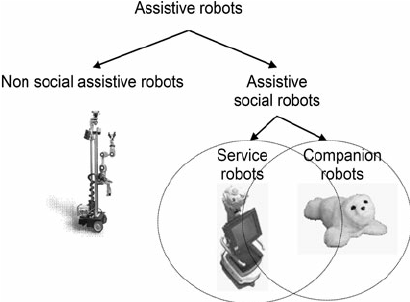
\includegraphics[scale=0.45]{gambar/kategori-assistive-robots.png}
  \caption{Pembagian kategori pada \emph{assistive robots} menurut \citet{cit:heerink2010}.}
  \label{fig:kategoriassistiverobots}
\end{figure}

Secara kategori, \citet{cit:heerink2010} membagi \emph{assistive robots} ke dalam dua kategori,
  yakni \emph{non social assistive robots} dan \emph{social assistive robots}.
Seperti yang terlihat pada gambar \ref{fig:kategoriassistiverobots},
\emph{non social assistive robots} mencakup robot yang digunakan untuk memberikan bantuan secara fisik kepada pengguna tanpa adanya interaksi sosial,
  sedangkan \emph{social assistive robots} mencakup robot yang melakukan tindakan \emph{assistive} dengan melibatkan interaksi sosial terhadap pengguna.
Lebih lanjut, \emph{social assistive robots} terbagi lagi ke dalam dua kategori,
  yakni \emph{service robots} dan \emph{companion robot}.
\emph{Service robots} merupakan robot yang memberikan bantuan fisik dan kognitif kepada pengguna,
  serta bertindak seolah sebagai pelayan,
  sedangkan \emph{companion robot} merupakan robot yang bertindak seolah sebagai pendamping,
  sahabat, dan media terapi secara sosial.

\subimport{1-assistive-robotics}{1-socially-assistive-robots.tex}
